\chapter{Analyse}
\label{analyse:chapter}

In diesem Kapitel werden folgende Fragen beantwortet:
\begin{itemize}
	\item \textit{''Wie funktioniert eine \gls{apt} Attacke und welche Schritte beinhaltet diese?''} - Abschnitt \ref{analyse:cc}
	\item \textit{''Was für Möglichkeiten bestehen, um HTTPS Verkehr unterbrechen zu können?''} - Abschnitt \ref{analyse:ssl}
	\item \textit{''Wie kann ein einzelner Netzwerkstrom, separiert von allen anderen, auf einen beliebigen Endpunkt dynamisch umgeleitet werden?''} - Abschnitt \ref{analyse:redirect}
	\item \textit{''Wie kann der HTTP/HTTPS Verkehr mitsamt Payload sauber geloggt werden?''} - Abschnitt \ref{analyse:logging}
	\item \textit{''Wie kann der HTTP/HTTPS Verkehr für die Analyse gespeichert werden?''} - Abschnitt \ref{analyse:database}
	\item \textit{''Wie kann die Malware anhand der gespeicherten Netzwerkpakete erkannt werden?''} - Abschnitt \ref{analyse:database}
	\item \textit{''Wie können die Angreifer und die Malware getäuscht werden?''} - Abschnitt \ref{analyse:fakecc}
\end{itemize}


%C&C
\section{Command \& Control}
\label{analyse:cc}
\subsection{Begrifflichkeit}
Der Begriff \gls{apt}\cite{wiki:apt} bezeichnet einen komplexen, zielgerichteten und effektiven Angriff auf kritische IT-Infrastrukturen. Bei solchen Angriffen gehen die Angreifer sehr zielgerichtet vor und nehmen grossen Aufwand auf sich. Das Ziel eines \gls{apt} ist es, möglichst lange unentdeckt  zu bleiben, um über längeren Zeitraum sensible Informationen auszuspähen oder Schaden anzurichten. Die Erkennung und Analyse dieser Angriffe gestalten sich als sehr schwierig. Nur das Sammeln, Analysieren und Korrelieren von Sicherheitsinformationen kann Hinweise zur Erkennung geben.

\subsection{Die 6 Schritte einer APT Attacke}
Die folgenden Punkte\cite{curthreat} beschreiben eine von vielen möglichen \gls{apt} Attacken. Es sind natürlich diverse andere Abläufe mit verschiedenen Zielen möglich.

\begin{enumerate}
	\item Der Angreifer schleust über einen beliebigen Attack Vector eine Malware in das Netzwerk einer Organisation ein. Das Netzwerk ist "compromised".
	\item Die Malware sucht nach weiteren Vulnerabilities oder kommuniziert mit command-and-control Servern, um Befehle oder Schadcode zu erhalten.
	\item Die Malware versucht Backdoors zu installieren, um den Angriff fortzusetzen, falls eine der Backdoors geschlossen wird.
	\item Wenn der Angreifer einen zuverlässigen Zugriff auf das Netzwerk der Organisation aufgebaut hat, können Benutzernamen und Passwörter gesammelt werden. Nun hat der Angreifer Zugriff auf die Systeme der Organisation.
	\item Die Malware sammelt Daten auf einem Staging Server und schleust die Daten dann aus dem Netzwerk der Organisation raus. Das Netzwerk ist "breached".
	\item Am Ende werden alle Beweise des Angriffs entfernt. Das Netzwerk bleibt jedoch "compromised", um den Angriff zu einem späteren Zeitpunkt fortzusetzen.
\end{enumerate}
%C&C

%Proxy
\section{Proxy}
\label{analyse:httpproxy}
\subsection{HTTP Proxy}
Ein HTTP Proxy\cite{wiki:proxy} erlaubt, den ein- und ausgehenden HTTP/HTTPS Verkehr über einen zentralen Punkt zu führen, das kann z.B. zum Filtern oder Sperren von nicht erlaubten Webseiten in einem Firmennetz interessant sein.
Der HTTP Proxy wird dabei nur über HTTP angesprochen, falls ein Client eine HTTPS Verbindung benötigt, wird dies über einen ''Proxy Connect'' \cite{rfc2817} gemacht, der eine \gls{ssl} Verbindung zur Zielseite aufbaut.
Die HTTPS Verbindung vom Client zum Server kann dabei nicht im Detail betrachtet werden, man sieht nur den Header, aber nicht den Body.
Bei einer reinen HTTP Verbindung ist ein ''Proxy Connect'' nicht nötig.

\begin{figure}[H]
	\centering
	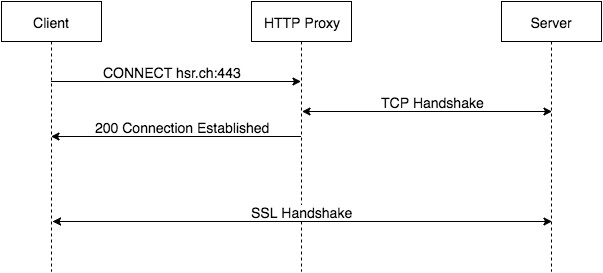
\includegraphics[width=\textwidth]{img/HTTP-Connect.png}
	\caption{Analyse: Proxy Connect}
	\label{fig:proxyconnect}
\end{figure}


\subsection{Proxy Framework}
Ein Proxy Framework bietet die Möglichkeit, einen eigenen Proxy und damit eine eigene Logik programmieren zu können, wie auf einen Request oder Response reagiert werden soll.
Die Proxy Frameworks sind oft zum Debuggen von Web Traffic gedacht, sie können aber auch für etwas ganz anderes verwendet werden, da die Logik selbst programmiert und angepasst werden kann.
Bekanntere Proxy Frameworks sind hierbei der MITMProxy\footnote{\url{https://mitmproxy.org/}} oder der FiddlerCore\footnote{\url{http://www.telerik.com/fiddler}}, beides sind Frameworks und können direkt in einem Software Projekt verwendet werden.

Die Evaluation der beiden Proxy Frameworks wurde im Abschnitt \ref{analyse:proxyframework} behandelt.

\newpage
\subsection{SSL Splitting}
\label{analyse:ssl}
\gls{ssl} Splitting\cite{sslsplit} ermöglicht die Einsicht in den Payload verschlüsselter Pakete.


\begin{figure}[H]
	\centering
	\includegraphics[width=\textwidth]{img/SSL-Splitting.png}
	\caption{Analyse: \gls{ssl} Splitting}
	\label{fig:sslsplitting}
\end{figure}

Das Einsehen von verschlüsseltem Traffic ist jedoch fragwürdig, da dadurch auch die Möglichkeit besteht, privaten Content zu protokollieren z.B. Passwörter.

\subsection{Evaluation Proxy Framework}
\label{analyse:proxyframework}


\begin{table}[H]
	\subsubsection{MITMProxy}
    \centering
	\begin{tabularx}{\textwidth}{| l | X | X |}
        \hline
        \textbf{Feature} & \textbf{Beschreibung} & \textbf{Bewertung} \\ \hline
        \textbf{Pattern Matching} & Zugriff auf Payload und Header. & \cellcolor{green!25}OK \\ \hline 
        \textbf{HTTP/S Verkehr umleiten} & Durch Umschreiben der Destination auf Layer 7 möglich.  & \cellcolor{green!25}OK \\ \hline 
        \textbf{SSL Splitting} & Wird unterstützt. & \cellcolor{green!25}OK \\ \hline 
        \textbf{Dokumentation} & Gut geschriebene Doku und einige Beispiele, welche allerdings nicht alle funktionieren. & \cellcolor{yellow!25}Genügend \\ \hline  
        \textbf{Entwicklungsstand} & Regelmässig neue Releases. & \cellcolor{green!25}OK \\ \hline
        \textbf{Performance} & Wird als interaktiver Proxy zu Debugzwecken und nicht als Proxy Library beworben. & \cellcolor{red!25}Ungenügend \\ \hline       
    \end{tabularx}
    \caption{Analyse: Prototyp V1 Evaluation MITMProxy}
\end{table}


\begin{table}[H]
	\subsubsection{FiddlerCore}
    \centering
	\begin{tabularx}{\textwidth}{| l | X | X |}
        \hline
        \textbf{Feature} & \textbf{Beschreibung} & \textbf{Bewertung} \\ \hline
        \textbf{Pattern Matching} & Zugriff auf Payload und Header & \cellcolor{green!25}OK \\ \hline 
        \textbf{HTTP/S Verkehr umleiten} & Durch Umschreiben der Destination auf Layer 7 möglich  & \cellcolor{green!25}OK \\ \hline 
        \textbf{SSL Splitting} & Wird unterstützt. & \cellcolor{green!25}OK \\ \hline 
        \textbf{Dokumentation} & Doku nur zu Klassen verfügbar, Beispiele sind meistens nur für die Skriptengine verfügbar, funktionieren jedoch auch mit FiddlerCore & \cellcolor{yellow!25}Genügend \\ \hline  
        \textbf{Entwicklungsstand} & Regelmässig neue Releases. & \cellcolor{green!25}OK \\ \hline
        \textbf{Performance} & Wird als Proxy Library für eigene Softwareprojekte beworben. & \cellcolor{green!25}OK \\ \hline       
    \end{tabularx}
    \caption{Analyse: Prototyp V1 Evaluation FiddlerCore}
\end{table}

\subsubsection{Schlussfolgerung}
Anhand der Evaluation in \ref{analyse:proxyframework} haben wir uns für die Proxy Library FiddlerCore entschieden, um den Prototyp V1 zu programmieren.

\subsection{Evaluation HTTP Proxy}

Beim HTTP Proxy wurden zwar bei der Analyse verschiedene Proxies (Privoxy \footnote{\url{https://www.privoxy.org/}}, Polipo\footnote{\url{https://www.irif.fr/~jch/software/polipo/}}) angeschaut, jedoch bietet nur der Squid Proxy \footnote{\url{http://www.squid-cache.org/}} von Haus aus einen \gls{icap} Client an (siehe \ref{analyse:icap}).

\subsubsection{Schlussfolgerung}
Wegen den in \ref{analyse:httpproxy} genannten Gründen hatten wir uns für den Squid Proxy entschieden, um den Prototyp V2 umzusetzen.


%Proxy


%Redirect
\section{Redirect}
\label{analyse:redirect}
\subsection{Iptables}
Iptables\cite{Iptables}\cite{wiki:iptables} ist eine Linux Applikation, die es ermöglicht, diverse Rules für die Linux Kernel Firewall zu definieren. Mit diesen Rules ist es möglich, anhand der Destination Adressen ein Paket auf eine andere Adresse umzuleiten. Dies geschieht auf Layer 3 und ist somit protokollunabhängig, was die darüber liegenden Layer bzw. Protokolle betrifft. Die Umleitung auf Layer 3 vereinfacht das System, da nicht auf Layer 7 diverse Ausnahmen, wie z.B. HTTP oder HTTPS, beachtet werden müssen.\\

Es gibt zwei mögliche Architekturen. Bei der ersten Variante wird die Iptable auf dem selben Host, auf dem auch der Proxy betrieben wird, gesetzt. Bei der zweiten Variante, befindet sich die Iptable auf einem anderen Host, der sich jedoch hinter dem Proxy befinden muss.

\subsubsection{Variante 1: Proxy und Iptables auf dem selben Host}

\begin{figure}[H]
	\centering
	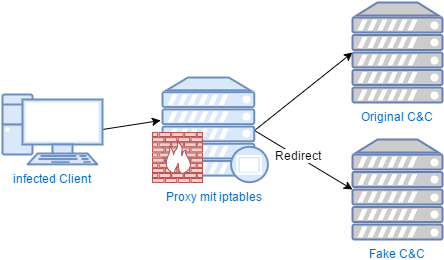
\includegraphics[width=\textwidth]{img/Redirect-attached.png}
	\caption{Analyse: Systemübersicht Variante 1}
	\label{fig:Systemübersicht: Variante 1, Proxy und Iptables auf dem selben Host}
\end{figure}

Zu beachten ist, dass die Pakete bei der INPUT Chain ankommen, da die Destination Adresse der Proxy ist. Das heisst, die Pakete werden wieder über die OUTPUT Chain ausgegeben. Die Iptable kann also wie unten beschrieben gesetzt werden um eine gewisse Destination Adresse auf eine andere umzuleiten. Bei dieser Architektur ist jedoch kein Proxy Chaining möglich, da bei einem Chaining die Destination immer die des nächsten Proxys ist.

\begin{listing}[H]
\begin{fancycode}
Iptables -t nat -A OUTPUT --destination [Original IP] -j DNAT --to-destination [Redirect IP]
\end{fancycode}
\caption{Analyse: Iptable Variante 1}
\label{lst:Iptable: Variante 1, Proxy und Iptables auf dem selben Host}
\end{listing}


\subsubsection{Variante 2: Proxy und Iptables auf separatem Host}

\begin{figure}[H]
	\centering
	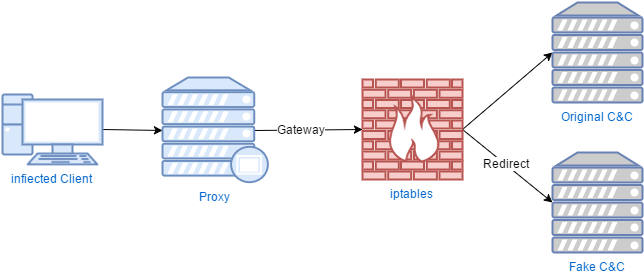
\includegraphics[width=\textwidth]{img/Redirect-detached.png}
	\caption{Analyse: Systemübersicht Variante 2}
	\label{fig:Systemübersicht: Variante 2, Proxy und Iptables auf separatem Host}
\end{figure}

Diese Architektur ist nur möglich, wenn der Host mit den Iptables als Gateway konfiguriert ist, da nur so die Pakete in der PREROUTING Chain ankommen. Das Masquerading wird benötigt, um die ursprüngliche Destination Adresse beim Response in die Source Adresse einzutragen, ansonsten lehnt der Client, der den Request gesendet hat, die Verbindung ab. Das Proxy Chaining kann umgangen werden, wenn die Iptables hinter oder auf dem letzten Proxy installiert werden.

\begin{listing}[H]
\begin{fancycode}
Iptables -t nat -A PREROUTING --destination [Original IP] -j DNAT --to-destination [Redirect IP]

Iptables -t nat -A POSTROUTING -j MASQUERADE
\end{fancycode}
\caption{Analyse: Iptable Variante 2}
\label{lst:Iptable: Variante 2, Proxy und Iptables auf separatem Host}
\end{listing}

\subsubsection{Schlussfolgerung}
Für die Realisierung des Prototyps V2 und der Fish Tank Suite fällt der Entscheid auf Variante 1, da sowohl Konfiguration als auch das Setup simpler ist. Mit Variante 2 ist es jedoch möglich, das Proxy Chaining zu umgehen, das in grösseren Firmennetzwerken unter Umständen notwendig ist.

\subsection{Layer 7 Redirect}
\label{analyse:layer7}
Bei einem Redirect auf Layer 7 wird der Header des HTTP/HTTPS Requests umgeschrieben, dabei wird ein Proxy Framework verwendet, welches diese Funktion im Normalfall anbietet. Es ist aber auch durch ein Rewrite-Programm\footnote{\url{http://www.squid-cache.org/Doc/config/url_rewrite_program/}} für einen HTTP Proxy möglich.

\begin{figure}[H]
	\centering
	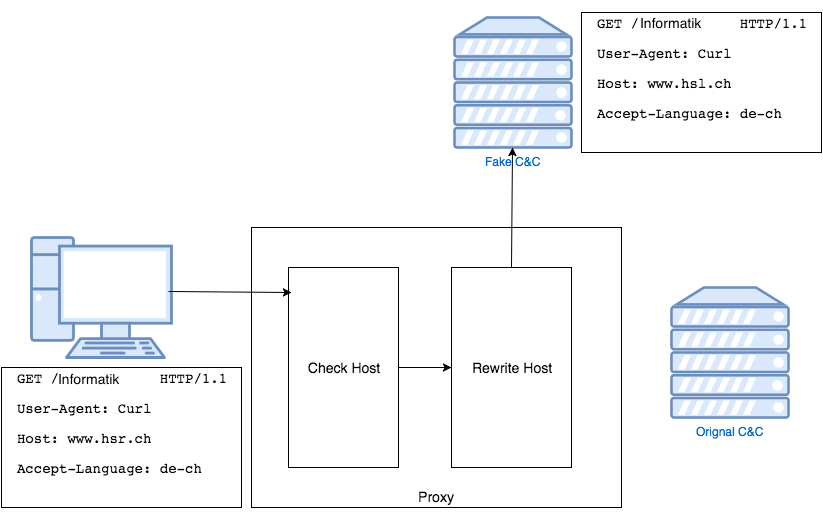
\includegraphics[width=\textwidth]{img/Layer7-Redirect.png}
	\caption{Analyse: Layer 7 Redirect}
	\label{fig:layer7redirect}
\end{figure}

\subsubsection{Schlussfolgerung}
Für die Realisierung des Prototyps V1 ist eine sofortige Umleitung vorgesehen, die nur mit dieser Methode möglich ist. Deshalb wird beim Prototyp V1 auf einen Layer 7 Redirect gesetzt.

%Redirect


%Logging
\section{Logging}
\label{analyse:logging}
\subsection{HTTP Proxy Logging}
HTTP Proxies\cite{squid:log} besitzen zwar Logging Möglichkeiten, jedoch hört dies bei Access Logs schon auf. Ganze Requests zu loggen gehört nicht zu den Logging-Möglichkeiten eines HTTP Proxies.

\subsection{Packetbeat}
Packetbeat\cite{elastic:packetbeat} \footnote{\url{https://www.elastic.co/products/beats/packetbeat}} ist ein Produkt von Elastic\footnote{\url{https://www.elastic.co}} und bietet das einfache Loggen von Netzwerk Paketen an.
Jedoch wird HTTPS als Protokoll nicht unterstützt und müsste durch eine eigene Implementation erweitert werden.


\subsection{TCPDump}
TCPDump\cite{tcpdump} \footnote{\url{http://www.tcpdump.org/tcpdump_man.html}} ist ein Programm um auf einem Port oder Interface zu horchen und alles was ankommt kann als PCAP Datei gespeichert werden, womit der ganze TCP Stream nachvollzogen werden kann. Allerdings ist die Lösung nur File-basiert und verschlüsselter Datenaustausch kann nicht inspiziert werden. 

\subsection{SSLDump}
SSLDump\cite{ssldump} \footnote{\url{http://ssldump.sourceforge.net/}} ist eine Erweiterung zu TCPDump und erlaubt das Entschlüsseln von verschlüsselten Paketen.


\subsection{\gls{icap}}
\label{analyse:icap}
\gls{icap}\cite{wiki:icap} wird verwendet, um HTTP Requests und Responses an einen Server weiterzuleiten, wo gewisse Änderungen, Malware Scans oder generelle Anpassungen gemacht werden können.
Dabei werden die bestehenden HTTP Requests und Responses in \gls{icap} Requests verpackt und als Body mitgesendet, falls nun SSL Splitting aktiviert ist, kann auch der Payload von verschlüsseltem Traffic auch auf einem ICAP Server angepasst werden.
\subsubsection{REQMOD}
Unter REQMOD versteht man die Request Modification, welche der \gls{icap} Client an den \gls{icap} Server sendet, dabei wird der ursprüngliche Request als Body in einen \gls{icap} Request eingebettet.
Der Server kann dann Modifikationen vornehmen und sendet die Requests zurück an den \gls{icap} Client.
\begin{figure}[H]
	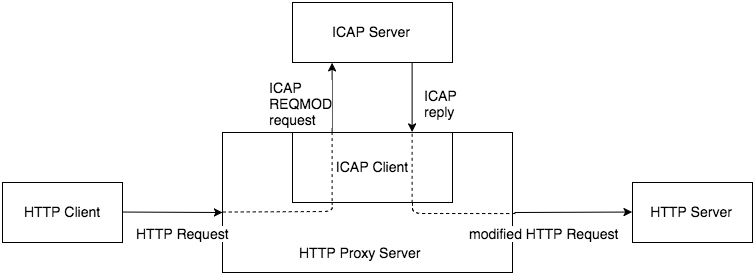
\includegraphics[width=\textwidth]{img/reqmod.png}
	\caption{Analyse: REQMOD Ablauf}
\end{figure}
\subsubsection{RESPMOD}
Unter RESPMOD versteht man die Response Modification, welche gleich wie REQMOD funktioniert, nur dass hierbei Responses modifiziert werden.
\begin{figure}[H]
	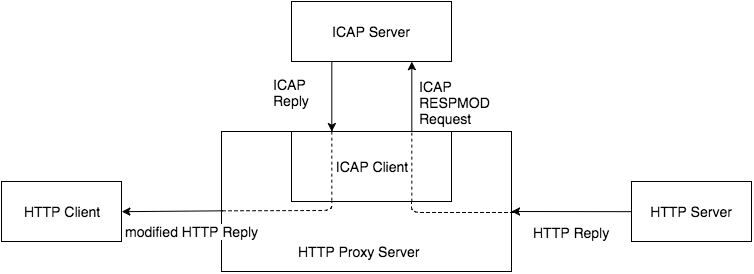
\includegraphics[width=\textwidth]{img/respmod.png}
	\caption{Analyse: RESPMOD Ablauf}
\end{figure}


\subsubsection{ICAP Client}
Der \gls{icap} Client kann ganze Request und Responses an den \gls{icap} Server senden oder aber er sendet nur eine Preview (bei Virus Checks kann dies reichen). Der Client sendet dazu eine OPTIONS Anfrage an den Server und bekommt zurück was er alles an den Server senden kann.
Die RESPMOD OPTIONS und REQMOD OPTIONS müssen einzeln abgefragt werden und können auch auf verschiedenen Servern aufgeschaltet werden.


\begin{listing}[H]
\begin{fancycode}
OPTIONS icap://icap.example.com/log_requests ICAP/1.0
Host: icap.example.com
\end{fancycode}
\caption{Analyse: ICAP Options Request}
\label{lst:icap-options-request}
\end{listing}

Anhand der \gls{icap} Responses auf die OPTIONS Anfrage, entscheidet der Client, ob er den ganzen Response bzw. Request sendet oder nur eine Preview.
Es kann auch eingeschränkt werden welche Methoden vom Server unterstützt sind.

\begin{listing}[H]
\begin{fancycode}
ICAP/1.0 200 OK
Date: Mon, 10 Nov 2016  09:55:21 GMT
Methods: RESPMOD
Service: ICAP Server
Encapsulated: null-body=0
Max-Connections: 100
Options-TTL: 3600
Transfer-Complete: 
Transfer-Ignore: jpg
\end{fancycode}
\caption{Analyse: ICAP Options Response}
\label{lst:icap-options-response}
\end{listing}


\subsubsection{ICAP Server}
Da der \gls{icap} Server keine Anpassungen am Body der Requests und Responses machen muss, können diese wieder ganz zurückgesendet werden, oder man sendet den Response 204 (No Modification Needed) an den \gls{icap} Client zurück.
Dabei kann auf dem \gls{icap} Server der ganze Request oder Response angeschaut und bei Bedarf auch irgendwohin geloggt werden zur weiteren Aufbereitung.



\subsection{Performance}
Weil beim Logging die Performance wichtig ist, da relativ viele Daten anfallen können, muss das Logging wenn möglich auf einen anderen Service ausgelagert werden, damit der Proxy seine Arbeit verrichten kann.

\subsection{Schlussfolgerung}
Da die Performance einer der wichtigsten Aspekte ist haben wir uns beim Logging für \gls{icap} entschieden, was eine Proxy unabhängige Lösung ist mit der Möglichkeit den Logging-Service woanders zu hosten.

%Logging

%Datenbank
\section{Datenbank}
\label{analyse:database}
\subsection{Elasticsearch}
Bei Elasticsearch\cite{elastic:elasticsearch}\footnote{\url{https://www.elastic.co/products/elasticsearch}} handelt es sich um ein \ac{fts} System, wodurch Suchen nach bestimmten Suchbegriffen oder Patterns in längeren Texten mit kleinem Zeitaufwand möglich ist.\\

Die Analyse der Datenhaltung ist nicht Teil der Arbeit. Es ist nur zu beachten, dass die gewählte Datenbank skalierbar ist, was auf Elasticsearch zutrifft.

\subsection{Kibana}
Kibana\cite{elastic:kibana}\footnote{\url{https://www.elastic.co/products/kibana}} ist ein Grafisches Dashboard für Elasticsearch, worauf man alle Einträge von Elasticsearch durchsuchen und visualisieren kann.

\begin{figure}[H]
	\centering
	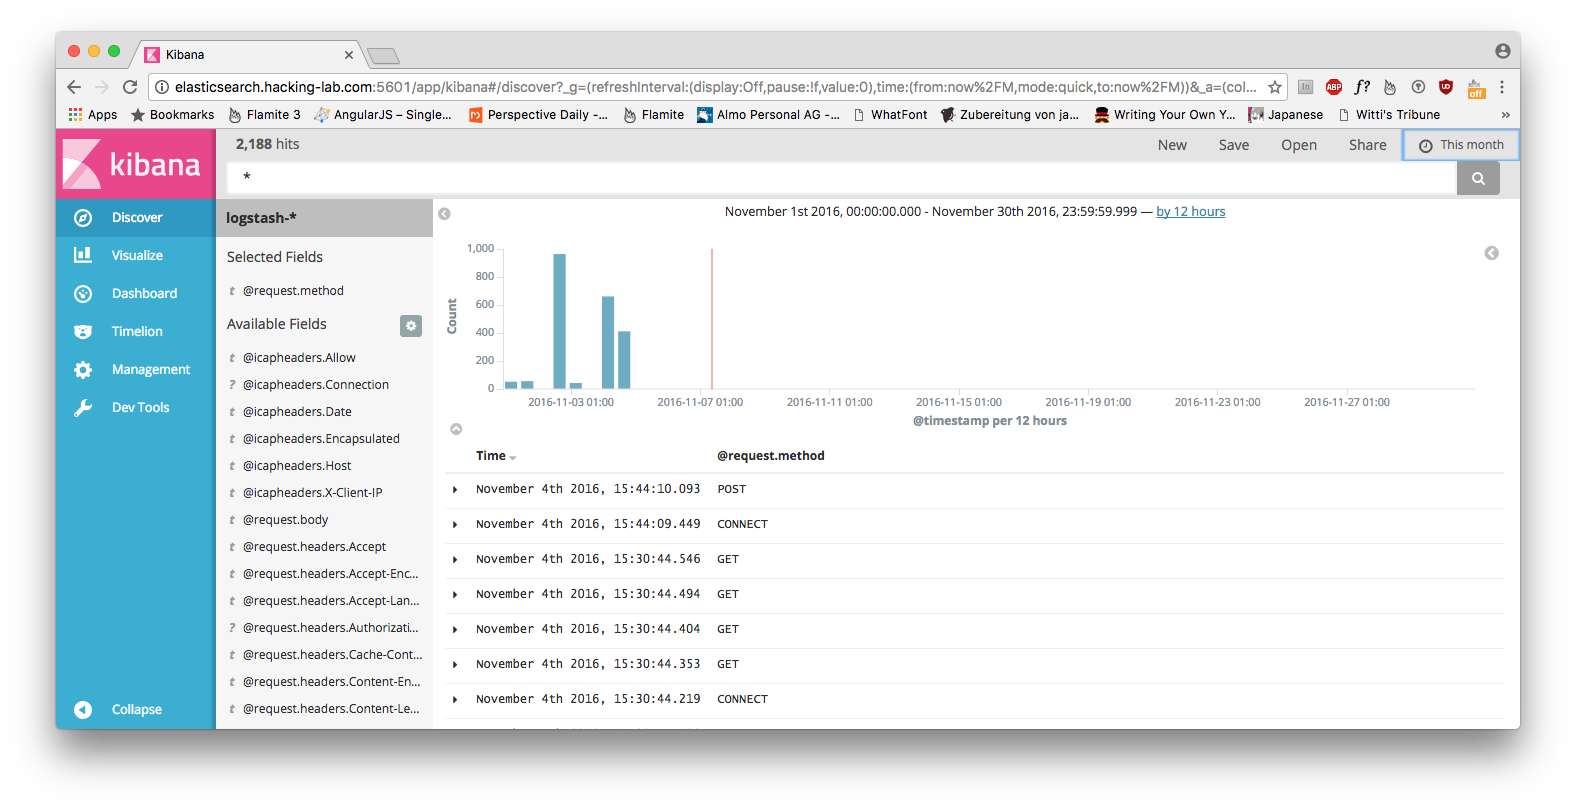
\includegraphics[width=\textwidth]{img/kibana}
	\caption{Analyse: Kibana Dashboard}
	\label{fig:kibana-dashboard}
\end{figure}
%Datenbank

%Malware Detetion
\section{Malware Detection}
\label{analyse:detection}
Die Erkennung der Malware kann auf verschiedenste Weise gelöst werden. Eine einfache Variante ist die Suche nach Schlüsselwörtern im Header und Payload. Es ist auch denkbar das Zeitverhalten beziehungsweise den Intervall von Paketen zu untersuchen und so Schlüsse auf Malware-Aktivitäten zu ziehen. Sicher ist, dass jede Malware seine ganz eigenen Eigenschaften besitzt, und nach diesen muss gezielt gesucht werden, das heisst eine generische Suche wäre zu ungenau.

\subsection{Pattern Matching im Payload}
Die Suche nach Schlüsselwörtern oder Patterns ist wie oben schon genannt die denkbar einfachste und auch präziseste Lösung. Es gibt jedoch ein grosses Problem bei diesem Verfahren. Der Payload könnte verschlüsselt sein. Falls es sich um eine symmetrische Verschlüsselung handelt kann der Key ermittelt werden, bei asymmetrischen Verschlüsselungen ist dies nicht so leicht. 

\subsubsection{Schlussfolgerung}
Diese Methode ist also nur möglich wenn der Payload im Klartext gelesen werden kann. Deswegen sind auch andere Erkennungsverfahren, bei denen der Payload keine Rolle spielt interessant.

\subsection{Zeitliches Verhalten}
Eine weitere Möglichkeit stellt das analysieren des zeitlichen Verhaltens gewisser Pakete dar. Dabei soll untersucht werden, ob eine Malware in gewissen abständen Pakete sendet.\\

In der Praxis stellt sich dieses Verfahren als sehr unpräzise dar, wenn man annimmt, dass nur das Zeitverhalten betrachtet werden darf und praktisch keine Informationen des Pakets zur Verfügung stehen. Das Problem dabei ist, dass bei einer Datenbankabfrage die Pakete im zeitlichen Abstand von 10 Sekunden liefern soll beinahe immer mehr als ein Paket pro Intervall zurückgeliefert wird. Das eigentliche Problem dabei ist nun die Assoziation der zusammengehörigen Pakete in den Intervalls, was schlichtweg unmöglich ist ohne weitere Parameter in den Algorithmus zu nehmen.

\begin{figure}[H]
	\centering
	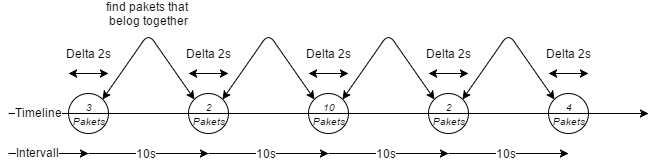
\includegraphics[width=\textwidth]{img/IntervallSearch.png}
	\caption{Analyse: Intervall Search}
	\label{fig:intervall_search}
\end{figure}


\subsubsection{Schlussfolgerung}
Die Analyse ergab, dass es zu viele False-Positives gibt, somit ist dieses Verfahren eher ungeeignet.

\subsection{URL Sequenz}
Dieses Verfahren baut auf der Analyse des zeitliche Verhaltens auf und versucht dessen Probleme zu verringern. Es geht hier darum durch eine Liste von URLs und die dazwischenliegenden ungefähren Zeitabstände das Verhalten einer Malware zu erkennen. Beim nachfolgenden Beispiel wird zuerst nach einem "register", und dann nach einem "hello" das 10 Sekunden später eingetroffen sein muss, gesucht.

\begin{enumerate}
	\item Suche nach Register-URI.
	\item Zeitpunkt der Register-URI merken.
	\item Suche nach der Hello-URI mit zeitlichem Offset nach dem Zeitpunkt der Register-URI.
	\item Falls die URIs im korrekten Abstand zueinander vorliegen handelt es sich um die Malware.
\end{enumerate}

\subsubsection{Schlussfolgerung}
Dieses Vorgehen ist um einiges genauer als nur der zeitliche Intervall. Es sind natürlich komplexere Abläufe denkbar, für die zur Verfügung gestellte Malware reicht das aber schon.

%Malware Detection


%Decryption
\section{Entschlüsselung}
Die Entschlüsselung ist in 3 Schritte aufgeteilt. Diese Schritte sind notwendig, um den verschlüsselten Payload in ein lesbares Format zu bringen. Die Schritte können bei anderen Verschlüsselungen anders ausfallen und können deshalb nicht generisch implementiert werden. Das heisst für jede Malware muss auch ein separater Algorithmus entwickelt werden.\\

Da die Malware für die die Entschlüsselungen entwickelt wurde vertraulich ist, können keine genauen Details über deren Funktionsweise dokumentiert werden.

\subsection{XOR und AES128}
\begin{enumerate}
	\item \textbf{EXTRACT:} Der Payload wird von unnötigen Zeichen befreit.
	\item \textbf{DECODE:} Der Text wird dekodiert (Base64).
	\item \textbf{DECRYPT:} Hier findet die eigentliche Entschlüsselung statt.
\end{enumerate}

\subsection{Logstash}
Bei Logstash\cite{elastic:logstash}\footnote{\url{https://www.elastic.co/products/logstash}} handelt es sich um eine Software, die das Zusammenfügen von Logs von verschiedenen Quellen sehr vereinfacht.
Dabei durchlaufen alle Logs im Normalfall die gleichen 3 Schritte.
\begin{enumerate}
	\item \textbf{INPUT:} Als Input können verschiedene Protokolle verwendet werden, an welche die Log Quellen ihre Logs senden.
	\item \textbf{FILTER:} Ein Filter wird zum Anreichern oder Anpassen der gesendeten Log Daten verwendet.
	\item \textbf{OUTPUT:} Zum Abschluss werden die Daten an einen Output gesendet, hier können ebenfalls verschiedene Protokolle verwendet werden oder eine Datenbank, wie zum Beispiel Elasticsearch.
\end{enumerate}



\subsection{Performance}
Da manchmal neue Entschlüsselungsalgorithmen entwickelt werden, muss Logstash nach der Aktualisierung neu gestartet werden.
Damit kein Unterbruch stattfindet, bis die Änderungen aufgeschaltet sind, bietet sich eine Queue an, die auch persistent bleibt, selbst wenn Logstash mal neu gestartet wird.

\subsection{Schlussfolgerung}
Da die Entschlüsselung von verschlüsseltem Payload zeitreibend ist, bietet es sich sehr an, diese auf einem eigenen Service vorzunehmen, um so allen anderen Systemen nicht in die Quere zu kommen.
Die Malware kann sich immer wieder ändern und dabei muss der Filter von Logstash upgedatet werden, daher wurde entschieden, eine RabbitMQ\cite{elastic:logstash:rabbitmq} Queue zwischen Log Quelle und Logstash zu setzen, damit keiner der Requests oder Responses verloren geht.


%Decryption


%Fake C&C
\section{Fake Command \& Control}
\label{analyse:fakecc}
Der Fake \gls{cc} befindet sich sobald eine Malware entdeckt wird immer wieder im Kontakt mit dem Original \gls{cc}, da dadurch sichergestellt werden kann, dass die Betreiber des Originalen \gls{cc} weniger schnell dahinter kommen, ob die Malware entdeckt wurde.
Die Malware sendet immer wieder Updates. Wenn nun der Redirect gesetzt ist, nimmt der Fake \gls{cc} den Request entgegen und leitet diesen an den Original \gls{cc} weiter.
Falls nun der Original \gls{cc} eine Antwort sendet entscheidet der Fake \gls{cc}, ob die Antwort weitergeleitet werden darf oder nicht.
Kurz gesagt der Fake \gls{cc} wird zur ''Fake Malware'' und behält den Original \gls{cc} bei Laune mit den weitergeleiteten Requests, zusätzlich wird der Malware vorgegaukelt, dass alles ok ist.

\begin{figure}[H]
	\centering
	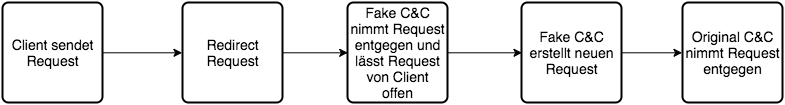
\includegraphics[width=\textwidth]{img/FakeCC-Request}
	\caption{Analyse: Fake C\&C Ablauf Request von Maleware}
	\label{fig:fakecc-request}
\end{figure}

\begin{figure}[H]
	\centering
	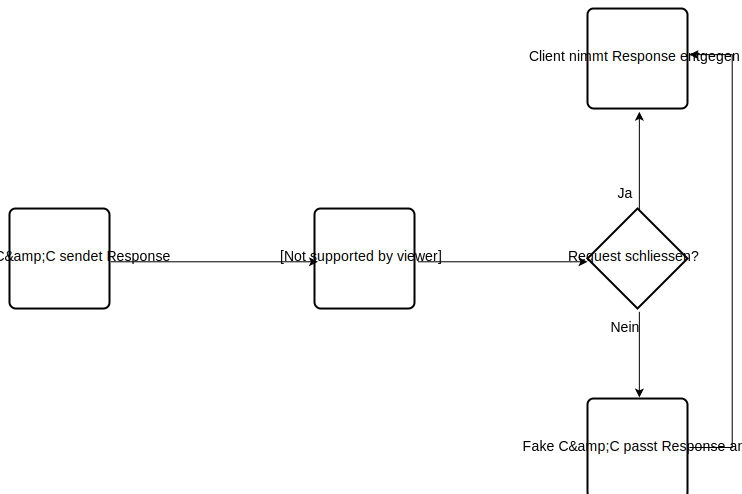
\includegraphics[width=\textwidth]{img/FakeCC-Response}
	\caption{Analyse: Fake C\&C Ablauf Response von Original \gls{cc}}
	\label{fig:fakecc-response}
\end{figure}

\subsection{Schlussfolgerung}
Mit diesem Verfahren bleibt der Original \gls{cc} immer aktuell und kein Verdacht tritt auf, dass die Requests der Malware über einen Fake \gls{cc} geleitet wurden.
Der Fake \gls{cc} kann so ebenfalls die Responses des Originalen \gls{cc} anpassen und bearbeiten.
%Fake C&C




